\documentclass[a4paper,10pt]{article}

\usepackage[english]{babel}
\usepackage[T1]{fontenc}
\usepackage[left=3cm, right=3cm, top=3cm, bottom=3cm]{geometry}
\usepackage{graphicx}
\usepackage[utf8]{inputenc}

%opening
\title{Labcontrol Manual}
\author{Markus Prasser}

\parindent 0pt
\parskip 12pt

\begin{document}

\maketitle

\tableofcontents

\newpage

\section{Introduction}

\emph{Labcontrol} is a tool to control a laboratory used for economic experiments with the software \emph{z-Tree}. This laboratory consists of a \emph{Linux} server and 18 \emph{Linux} clients used to conduct those experiments. The primary functions of \emph{Labcontrol} are the startup and management of experiment sessions, automated receipts printing and easy administration of the clients.

\begin{center}
  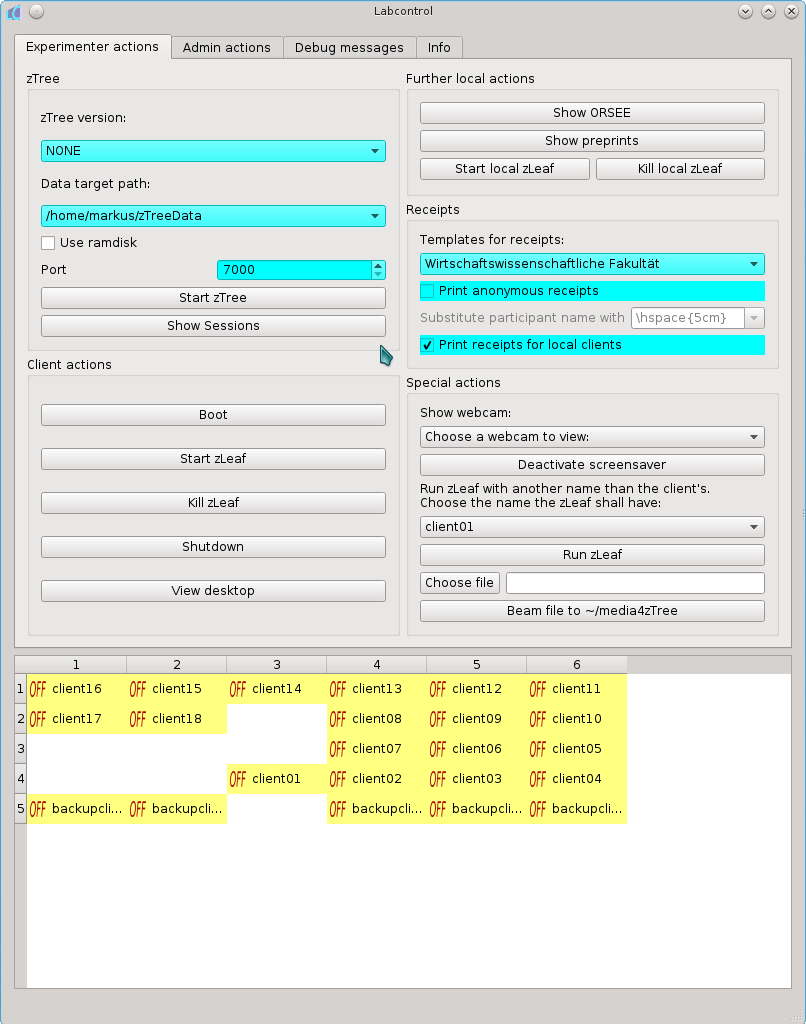
\includegraphics[scale=.4]{pictures/startup_screen.png}
\end{center}

\subsection{Working Features}

\begin{itemize}
  \item A \emph{Qt5} GUI for experiments and administration showing the clients' current states
  \item boot and shutdown the clients, start and kill \emph{z-Leaves} on them using \emph{ssh}
  \item detect all installed \emph{z-Tree} versions
  \item automatic receipts printing after creation of the payment file by \emph{z-Tree}
  \item beam media files to the clients using \emph{rcp}
  \item watch clients' desktops using \emph{VNC}
  \item open external programs showing the laboratories' webcams
  \item execute admin functions on the clients
  \item automatic and regular querying of the clients' statuses using \emph{ping} and \emph{netstat}
  \item simultaneous running of multiple \emph{z-Tree} instances on different ports
  \item administrator and experiment users with different privileges
\end{itemize}

\subsection{Wish-list}

\begin{itemize}
  \item logging support for a better overview over experiments and error discovery in the laboratory
  \item integration into \emph{ORSEE} for automated experiment finishing
  \item improve handling of multiple concurrent sessions, currently just viewing them is supported
\end{itemize}

\section{Requirements}

Labcontrol was designed and programmed to be as error insensitive as possible. Even with all data and settings (except the executable of course) missing it should still be able to start up and run. Only the functionality will be very limited. This was made to make installing and testing as easy as possible by allowing a step by step approach.

\subsection{Files And Basic Environment}

\emph{Labcontrol} was tried to be programmed as versatile as possible, e.g. all important paths are configurable with \emph{Qt}'s QSettings configuration system. Also we tried to include no compilation time dependencies except \emph{Qt5}.
\begin{itemize}
  \item Your setup should consist of a server running \emph{z-Tree} and clients to run the \emph{z-Leaves}.
  \item Our laboratory works fine using \emph{Debian Jessie} with a self compiled \emph{wine} in version 1.4.1.
  \item All clients should be listed in \texttt{/etc/hosts} on the server and the server on the clients. For most functions the IP addresses are used directly, but the status querying relies on hostnames.
  \item All clients should have a special user dedicated for experiments. Since \emph{Labcontrol} uses \emph{ssh}, password-less public-key authentication must be available at least for the user. For administrative tasks on the client also \texttt{root} must be available for public-key authentication.
  \item All \emph{z-Tree} and \emph{z-Leaf} executables should be stored in a central folder on the server and the clients with each version in a separate folder following the naming scheme \texttt{zTree\_X.Y.Z}, otherwise the automatic detection will not work.
  \item The directories in the \texttt{data} directory should be copied to the so called \emph{labcontrol installation directory}, both on the server and the clients.
  \item The \texttt{Labcontrol.conf} file should be copied to the place where \emph{Qt} stores the \emph{QSetting}s files (on \emph{Linux} this should be \texttt{/etc/xdg/Economic\ Laboratory}). Afterwards it should be adjusted to match the laboratory's specifications.
  \item To automatically deploy media files on the clients in the client's experiment user's home directory there should be a read-write accessible directory \texttt{media4ztree}
\end{itemize}

\subsection{External Runtime Dependencies}

\begin{itemize}
  \item on \emph{Linux} \emph{wine} to run the \emph{z-Tree} and \emph{z-Leaf} binaries
  \item a wake-on-lan program for remote client startup
  \item public-key enabled \emph{ssh} access to the clients
  \item optionally a \emph{VNC} client to show the clients' desktops (and a \emph{VNC} server on them)
  \item a web browser to show \emph{ORSEE}
  \item \emph{latex}, \emph{dvips}, \emph{ps2pdf} and \emph{lpr} for automatic receipts creation and printing
  \item a postscript viewer to display the generated receipts
\end{itemize}

\section{Compilation And Installation}

To compile Labcontrol it should be sufficient to open the \texttt{Labcontrol.pro} file with \emph{Qt Creator} and compile after choosing the desktop profile.

In the compilation process a special build directory will be created in which the compiled executable will be found after successfull compilation. You can place this executable anywhere you want. On \emph{Linux} we suggest to place it in \texttt{/usr/local/bin}. \emph{Linux} users also can use the supplied \texttt{labcontrol.desktop} file and place it in \texttt{/usr/share/applications} to have an accessible desktop icon.

Like already mentioned all \emph{z-Tree} and \emph{z-Leaf} versions should be copied to a central directory, the \emph{zTree installation directory}. This directory will be automatically scanned for installed \emph{z-Tree} versions by searching for folders matching the pattern \texttt{zTree\_X.Y.Z}.

The directories in the \texttt{data} directory should be copied to the \emph{zTree installation directory}.

Afterwards place the \texttt{Labcontrol.conf} in a subfolder \texttt{Labcontrol} in the place where \emph{QSettings} stores its definitions on your platform (on \emph{Linux} this would be \texttt{/etc/xdg/Labcontrol/Labcontrol.conf}) and adjust it to your needs and prerequisites.

To allow \emph{Labcontrol} to control the clients password-less public-key authentication must be available at least for the experiment user on the clients. For administration this is also required for \texttt{root}. Also all clients should be known by \texttt{ /etc/ssh/ssh\_known\_hosts}. This file must be readable by the users! If this is missing \emph{Labcontrol} will query the user on every connection attempt, which is not user-friendly.

\section{Using Labcontrol}

After startup \emph{Labcontrol} initializes all available components and loads its settings stored in \emph{QSettings}. On any possible error \emph{Labcontrol} will display an error message what type of error occurred and what consequences it has for the functionality of \emph{Labcontrol}.

Afterwards \emph{Labcontrol} will greet the user with its main window. This consists of a table view at the bottom showing all known clients and their current states. This view may take some seconds to initialize depending on the time it takes to query the initial client statuses. In the upper area there is a tabbed area consisting of three tabs. Most users will only use the \emph{Experimenter actions} tab which hosts all options needed to conduct experiments. Only admins are allowed to use the \emph{Admin actions} tab, which will be deactivated for all other users. The \emph{Debug messages} tab does exactly what its title says: display debug messages. It's useful for checking configuration and other errors but is of no interest for normal users. At last license and building information will be shown in the \emph{Info} tab.

\subsection{The Experimenter actions tab}

This tab consists of five group boxes grouping tasks and options of one kind. The first one is the \emph{z-Tree} one. Before you start a session you need to choose a particular z-Tree version, the port you want to use and where the data shall be stored. If this path does not exist it will be created by \emph{Labcontrol}. Since this path will be passed to \emph{z-Tree} please do not use any special characters of spaces in it. Otherwise there will be the possibility of data loss. After all settings where done \emph{z-Tree} can be started by clicking the respective button. Because of the possibility to run multiple simultaneous sessions (which likewise means \emph{z-Tree} instances) a function to display all active sessions was also implemented. It allows no modifications but just the display of currently running sessions.

To the start of a session is also bound the start of all receipts printing facilities. So users are strongly advised not to kill \emph{Labcontrol} while conducting a session because then the automated receipts printing will not work. \emph{z-Tree} is always started as a stand-alone program so killing \emph{Labcontrol} or a crash of it will mean no harm to \emph{z-Tree}.

The \emph{Client actions} and \emph{Further local options} group boxes are self explanatory.

Another important group box for the sessions is the \emph{Receipts} group box. All settings made there apply to the next started session and cannot be altered after starting a session. The user is able to choose between several installed receipt templates (if there are any installed) and can optionally make the receipts anonymous. If the user chooses to do so he is also able to choose the string which shall replace the user name. Printing receipts for local clients (\emph{z-Leaf} instances on the server) can be deactivated. This only works if the name given to the local client contains the string \texttt{local}. Also the user should take care, that none of the participants has \texttt{local} in his name, because then this participant would not get a receipt generated.

The last one is the \emph{Special actions} group box. This allows you to choose a webcam to show. After choosing a webcam an external program will open showing a window with the cameras view. Second there is a button to manually deactivate the screen savers of the clients. In some cases (e.g. replacing a client with a maintenance one) \emph{z-Leaves} can be started with others names than their own client's host name. To do this the user can choose the name of any client and afterwards click the \emph{Run z-Leaf} button. Last there is the option to beam files to an already existing directory \texttt{media4ztree} in the client user's home directory. All files which shall be beamed should be placed in one folder. The folder name and the in it contained files' names should also include no special characters of spaces.

\subsection{The Admin actions tab}

This tab allows to do some administrative tasks. The user can open terminals or file managers connected to the clients. Also specific commands can be run for the entire laboratory.

\subsection{The Debug messages tab}

This tab is very useful for installing and debugging. All configuration options get listed there and if you run a command or click a button (e.g. the "`Start z-Leaf"' button) the command behind this function is displayed there, so you can copy and paste it into a terminal and check there, why it is not working.

\end{document}
